\section{\propMatricesTitle} \label{properties_matrices}


\begin{definition}
An $r\times k$ matrix\index{Matrix} $M=(m^i_j)$ for $i=1, \ldots, r; j=1, \ldots, k$ is a rectangular array of real (or complex) numbers:
\label{matrixnotation}
\[M = 
\begin{pmatrix}
m_1^1 & m_2^1 & \cdots & m_k^1 \\
m_1^2 & m_2^2 & \cdots & m_k^2 \\
\vdots & \vdots &   & \vdots \\
m_1^r & m_2^r & \cdots & m_k^r \\
\end{pmatrix}
\]
The numbers $m^i_j$ are called \emph{entries}\index{Matrix!entries of}.  The superscript indexes the row of the matrix and the subscript indexes the column of the matrix in which $m_j^i$ appears\footnote{This notation was first introduced by Albert Einstein.}.
\end{definition}

%It is often useful to consider matrices whose entries are more general than the real numbers, so we allow that possibility.

An $r\times 1$ matrix $v = (v^r_1) = (v^r)$ is called a \emph{column vector}\index{Column vector}, written \[v = \colvec{v^1\\v^2\\ \vdots \\ v^r }\, .\]  A $1\times k$ matrix $v = (v^1_k) = (v_k)$ is called a \emph{row vector}\index{Row vector}, written \[v = \rowvec{v_1 & v_2 & \cdots & v_k }\, .\]  


Matrices are a very useful and efficient way to store information:

\begin{example}
In computer graphics, you may have encountered image files with a .gif extension.  These files are actually just matrices: at the start of the file the size of the matrix is given, and then each entry of the matrix is a number indicating the color of a particular pixel in the image.

The resulting matrix  then has its rows shuffled a bit: by listing, say, every eighth row, then a web browser downloading the file can start displaying an incomplete version of the picture before the download is complete.

Finally, a compression algorithm is applied to the matrix to reduce the size of the file.
\end{example}

\videoscriptlink{matrices_example.mp4}{Adjacency Matrix Example}{scripts_matrices_example}

\begin{example}
Graphs occur in many applications, ranging from telephone networks to airline routes.  In the subject of \emph{graph theory}\index{Graph theory}, a graph is just a collection of vertices and some edges connecting vertices.  A matrix can be used to indicate how many edges attach one vertex to another.

\begin{center}
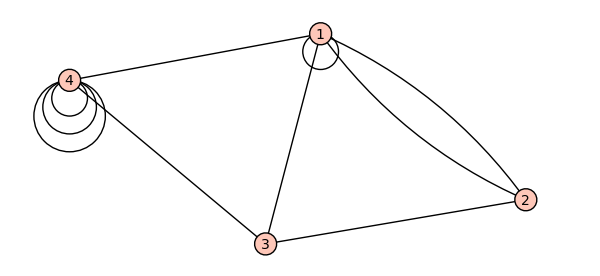
\includegraphics[width=10cm]{notes8-0.png}
\end{center}
For example, the graph pictured above would have the following matrix, where $m^i_j$ indicates the number of edges between the vertices labeled $i$~and~$j$:
\[
M = \begin{pmatrix}
1 & 2 & 1 & 1 \\
2 & 0 & 1 & 0 \\
1 & 1 & 0 & 1 \\
1 & 0 & 1 & 3 \\
\end{pmatrix}
\]
This is an example of a \emph{symmetric matrix}, since $m_j^i = m_i^j$.
\end{example}

The space of $r\times k$ matrices $M_k^r$ is a vector space with the addition and scalar multiplication defined as follows:
\begin{align*}
&M+N = (m_j^i) + (n_j^i) = ( m_j^i + n_j^i ) \\
&rM = r(m_j^i) = (rm_j^i)
\end{align*}
In other words, addition just adds corresponding entries in two matrices, and scalar multiplication multiplies every entry.
Notice that $M_1^n = \mathbb{R}n$ is just the vector space of column vectors.

Recall that we can multiply an \(r \times k\) matrix by a \(k \times 1\) column vector to produce a \(r \times 1\) column vector using the rule
\[MV = \big(\sum_{j=1}^k m_j^i v^j\big)\, .\]

This suggests a rule for multiplying an \(r \times k\) matrix \(M\) by a \(k \times s\) matrix~\(N\): our \(k \times s\) matrix \(N\) consists of \(s\) column vectors side-by-side, each of dimension \(k \times 1.\) We can multiply our \(r \times k\) matrix \(M\) by each of these \(s\) column vectors using the rule we already know, obtaining \(s\) column vectors each of dimension \(r \times 1.\) If we place these \(s\) column vectors side-by-side, we obtain an \(r \times s\) matrix \(MN.\)

That is, let \[N = 
\begin{pmatrix}
n_1^1 & n_2^1 & \cdots & n_s^1 \\
n_1^2 & n_2^2 & \cdots & n_s^2 \\
\vdots & \vdots &   & \vdots \\
n_1^k & n_2^k & \cdots & n_s^k \\
\end{pmatrix}
\]
and call the columns \(N_1\) through \(N_s\):
\[N_1 = \colvec{n_1^1\\n_1^2\\\vdots\\n_1^k},
N_2 = \colvec{n_2^1\\n_2^2\\\vdots\\n_2^k},
\ldots,
N_s = \colvec{n_s^1\\n_s^2\\\vdots\\n_s^k}.
\]
Then
%\[
%MN=M \rowvec{N_1 & N_2 & \cdots & N_s} = \rowvec{MN_1 & MN_2 & \cdots & MN_s}.
%\]%
\[
MN=M
\begin{pmatrix}
| & | & & | \\
N_1 & N_2 & \cdots & N_s \\
| & | & & | \\
\end{pmatrix}
=
\begin{pmatrix}
| & | & & | \\
MN_1 & MN_2 & \cdots & MN_s \\
| & | & & | \\
\end{pmatrix}
\]

A more concise way to write this rule is: If \(M=(m^i_j)\) for \(i=1, \ldots, r; j=1, \ldots, k\) and \(N=(n^i_j)\) for \(i=1, \ldots, k; j=1, \ldots, s,\) then \(MN=L\) where \(L=(\ell^i_j)\) for \(i=i, \ldots, r; j=1, \ldots, s\) is given by
\[
\ell^i_j = \sum_{p=1}^k m^i_p n^p_j.
\]
This rule obeys linearity.

Notice that in order for the multiplication to make sense, the columns and rows must match.  For an $r\times k$ matrix $M$ and an $s\times m$ matrix $N$, then to make the product $MN$ we must have $k=s$.  Likewise, for the product $NM$, it is required that $m=r$.  A common shorthand for keeping track of the sizes of the matrices involved in a given product is: 
\[\Big(r \times k\Big)\times \Big(k\times m\Big) = \Big(r\times m\Big)\]

\begin{example}
Multiplying a $(3\times 1)$ matrix and a $(1\times 2)$ matrix yields a $(3\times 2)$ matrix.
\[
\colvec{1\\3\\2} \rowvec{2 & 3} = 
\begin{pmatrix}
1\cdot 2 & 1\cdot 3 \\
3\cdot 2 & 3\cdot 3 \\
2\cdot 2 & 2\cdot 3 \\
\end{pmatrix}
= \begin{pmatrix}
2 & 3 \\
6 & 9 \\
4 & 6 \\
\end{pmatrix}
\]
\end{example}

\begin{center}\href{\webworkurl ReadingHomework8/1/}{Reading homework: problem 8.1}\end{center}

Recall that $r\times k$ matrices can be used to represent linear transformations 
$ \mathbb{R}k \rightarrow \mathbb{R}r $
via \[MV = \sum_{j=1}^{k} m_j^iv^j , \] which is the same rule we use when we multiply an $r\times k$ matrix by a $k\times 1$ vector to produce an $r\times1$ vector.

Likewise, we can use a matrix $N=(n^i_j)$ to represent a linear transformation
\[
L \colon M^s_k \stackrel{N}{\longrightarrow} M^r_k
\]
via 
\[
L(M)^i_l = \sum_{j=1}^{s} n_j^im^j_l.
\]
This is the same as the rule we use to multiply matrices. \hypertarget{leftmult}{In other words,} \(L(M)=NM\) is a linear transformation.

\begin{definition}[Matrix Terminology]
The entries $m_i^i$ are called \emph{diagonal}, and the set $\{m_1^1$, $m_2^2$, $\ldots \}$~is called the \emph{diagonal of the matrix}\index{Matrix!diagonal of}.

Any $r\times r$ matrix is called a \emph{square matrix}\index{Square matrix}.  A square matrix that is zero for all non-diagonal entries is called a diagonal matrix\index{Diagonal matrix}.

The $r\times r$ diagonal matrix with all diagonal entries equal to $1$ is called the \emph{identity matrix}\index{Identity matrix}, $I_r$, or just $\1$.  An identity matrix looks like \[
\begin{pmatrix}
1 & 0 & 0 & \cdots & 0 \\
0 & 1 & 0 & \cdots & 0 \\
0 & 0 & 1 & \cdots & 0 \\
\vdots & \vdots & \vdots & \ddots & \vdots \\
0 & 0 & 0 & \cdots & 1
\end{pmatrix}.
\]
The identity matrix is special because \[I_rM=MI_k=M\] for all $M$ of size $r\times k$.
\end{definition}

In the matrix given by the product of matrices  above, the diagonal entries are $2$ and $9$.
An example of a diagonal matrix is 
\[\begin{pmatrix}
2 & 0 & 0\\
0 & 3 & 0\\
0 & 0 & 0\\
\end{pmatrix}\, .\]

\begin{definition}
The \emph{transpose}\index{Transpose} of an $r\times k$ matrix $M = (m_j^i)$ is the $k\times r$ matrix with entries
\[
M^T = (\hat{m}_j^i)
\]
with $\hat{m}_j^i = m_i^j$. 

A matrix $M$ is \emph{symmetric}\index{Symmetric matrix} if $M=M^T$.
\end{definition}

\begin{example}
$\begin{pmatrix}
2 & 5 & 6\\
1 & 3 & 4\\
\end{pmatrix}^T = 
\begin{pmatrix}
2 & 1 \\
5 & 3 \\
6 & 4 \\
\end{pmatrix}$
\end{example}

\begin{center}\href{\webworkurl ReadingHomework8/2/}{Reading homework: problem 8.2}\end{center}

\begin{remark}[Observations]

$\phantom{test}$

\begin{itemize}
\item Only square matrices can be symmetric.

\item The transpose of a column vector is a row vector, and vice-versa. 

\item Taking the transpose of a matrix twice does nothing.  \emph{i.e.,} $(M^T)^T=M$.
\end{itemize}
\end{remark}

\begin{theorem}[Transpose and Multiplication]
Let $M, N$ be matrices such that $MN$ makes sense.  Then $(MN)^T = N^TM^T$.
\end{theorem}
The proof of this theorem is left to \hyperref[MN=NTMT]{Review Question~\ref*{MN=NTMT}}.

Sometimes matrices do not share the properties of regular numbers, watch this video to see why:

\videoscriptlink{matrices_commute.mp4}{Matrices do not Commute}{script_matrices_commute}

Many properties of matrices following from the same property for real numbers. Here is an example.

\begin{example}
{\itshape Associativity of matrix multiplication.} We know for real numbers $x$, $y$ and $z$ that 
\[
x(yz)=(xy)z\, ,
\]
{\itshape i.e.} the order of bracketing does not matter. The same property holds for matrix multiplication, let us show why.
Suppose $M=\big( m^i_j \big)$, $N=\big( n^j_k \big)$ and  $R=\big( r^k_l \big)$ are, 
respectively, $m\times n$, $n\times r$ and $r\times t$ matrices. Then from the rule for matrix
multiplication we have
\[
MN=\Big(\sum_{j=1}^n m^i_j n^j_k\Big)\mbox{ and } NR=\Big(\sum_{k=1}^r n^j_k r^k_l\Big)\, .
\]
So first we compute 
\[
(MN)R=\Big(\sum_{k=1}^r \Big[\sum_{j=1}^n m^i_j n^j_k\Big] r^k_l \Big) = 
\Big(\sum_{k=1}^r \sum_{j=1}^n \Big[ m^i_j n^j_k\Big] r^k_l \Big) =\Big(\sum_{k=1}^r \sum_{j=1}^n m^i_j n^j_k r^k_l \Big)\, .
\]
In the first step we just wrote out the definition for matrix multiplication, in the second step we
moved summation symbol outside the bracket (this is just the distributive
property $x(y+z)=xy+xz$ for numbers) and
in the last step we used the associativity property for real numbers to remove the square brackets. 
Exactly the same reasoning shows that
\[
M(NR)=\Big(\sum_{j=1}^n m^i_j\Big[\sum_{k=1}^r n^j_k r^k_l\Big]\Big) = 
\Big(\sum_{k=1}^r \sum_{j=1}^n  m^i_j \Big[n^j_kr^k_l \Big] \Big) =\Big(\sum_{k=1}^r \sum_{j=1}^n m^i_j n^j_k r^k_l \Big)\, .
\]
This is the same as above so we are done. {\itshape As a fun remark, note that Einstein would simply have written
$(MN)R=(m^i_j n^j_k) r^k_l= m^i_j n^j_k r^k_l = m^i_j (n^j_k r^k_l ) = M(NR)$.}
\end{example}


\subsection{Block Matrices}

It is often convenient to partition a matrix $M$ into smaller matrices called \emph{blocks}, like so:
\[
M=\begin{pmat}{ccc|c}
1 & 2 & 3 & 1 \\
4 & 5 & 6 & 0 \\
7 & 8 & 9 & 1 \\
\cline{1-4}
0 & 1 & 2 & 0 \\
\end{pmat}
=
\begin{pmat}{c|c}
A & B \\
\cline{1-2}
C & D \\
\end{pmat}
\]
Here $A = \begin{pmatrix}
1 & 2 & 3 \\
4 & 5 & 6 \\
7 & 8 & 9 \\
\end{pmatrix}$, $B=\colvec{1\\0\\1}$, $C=\rowvec{0 & 1 & 2 }$, $D=(0)$.

\begin{itemize}
\item The blocks of a block matrix\index{Block matrix}  must fit together to form a rectangle.  So 
$\begin{pmat}{c|c}
B & A \\
\cline{1-2}
D & C \\
\end{pmat}
$ makes sense, but 
$\begin{pmat}{c|c}
C & B \\
\cline{1-2}
D & A \\
\end{pmat}
$ does not.

%\href{\webworkurl ReadingHomework9/1/}{Reading homework: problem 9.1}
\reading{9}{1}

\item There are many ways to cut up an $n\times n$ matrix into blocks.  Often context or the entries of the matrix will suggest a useful way to divide the matrix into blocks.  For example, if there are large blocks of zeros in a matrix, or blocks that look like an identity matrix, it can be useful to partition the matrix accordingly.

\item Matrix operations on block matrices can be carried out by treating the blocks as matrix entries.  In the example above,
\begin{align*}
M^2 & = \begin{pmat}{c|c}
A & B \\
\cline{1-2}
C & D 
\end{pmat}
\begin{pmat}{c|c}
A & B \\
\cline{1-2}
C & D 
\end{pmat} \\
& = \begin{pmat}{c|c}
A^2+BC & AB+BD \\
\cline{1-2}
CA+DC & CB+D^2
\end{pmat} 
\end{align*}

Computing the individual blocks, we get:
\begin{align*}
A^2+BC &= \begin{pmatrix}
	30 & 37 & 44 \\
	66 & 81 & 96 \\
	102&127 &152 
	\end{pmatrix} \\
AB+BD  &=\colvec{ 4 \\ 10 \\ 16 } \\
CA+DC  &=\rowvec{ 18 \\ 21 \\ 24 } \\
CB+D^2 &=(2) 
\end{align*}

Assembling these pieces into a block matrix gives:
\[
\begin{pmat}{ccc|c}
30 & 37 & 44 & 4 \\
66 & 81 & 96 & 10 \\
102 & 127 & 152 & 16 \\
\cline{1-4}
4 & 10 & 16 & 2 \\
\end{pmat}
\]

This is exactly $M^2$.
\end{itemize}

\subsection{The Algebra of Square Matrices }\index{Square matrices}

Not every pair of matrices can be multiplied.  When multiplying two matrices, the number of rows in the left matrix must equal the number of columns in the right.  For an $r\times k$ matrix $M$ and an $s\times l$ matrix $N$, then we must have~$k=s$.

This is not a problem for square matrices of the same size, though.  Two $n\times n$ matrices can be multiplied in either order.  For a single matrix $M \in M^n_n$, we can form $M^2=MM$, $M^3=MMM$, and so on, and define $M^0=I_n$, the identity matrix.

As a result, any polynomial equation can be evaluated on a matrix.

\begin{example}
Let $f(x) = x - 2x^2 + 3x^3$.

Let $M=\begin{pmatrix}
1 & t \\
0 & 1 \\
\end{pmatrix}$.  Then:
\[
M^2 = \begin{pmatrix}
1 & 2t \\
0 & 1 \\
\end{pmatrix},
M^3 = \begin{pmatrix}
1 & 3t \\
0 & 1 \\
\end{pmatrix}, \ldots
\]

Hence:
\begin{align*}
f(M) &=\begin{pmatrix}
	1 & t \\
	0 & 1
	\end{pmatrix} 
- 2 \begin{pmatrix}
	1 & 2t \\
	0 & 1
	\end{pmatrix} 
+ 3 \begin{pmatrix}
	1 & 3t \\
	0 & 1
	\end{pmatrix} \\
&= \begin{pmatrix}
	2 & 6t \\
	0 & 2
	\end{pmatrix}
\end{align*}
\end{example}

Suppose $f(x)$ is any function defined by a convergent Taylor Series:
\[
f(x) = f(0) + f'(0)x + \frac{1}{2!}f''(0)x^2 + \cdots
\]
Then we can define the matrix function by just plugging in $M$:
\[
f(M) = f(0) + f'(0)M + \frac{1}{2!}f''(0)M^2 + \cdots
\]
There are additional techniques to determine the convergence of Taylor Series of matrices, based on the fact that the convergence problem is simple for diagonal matrices.  It also turns out that $\exp (M) = 1 + M + \frac{1}{2}M^2 + \frac{1}{3!}M^3 + \cdots$ always converges.

\videoscriptlink{properties_of_matrices_example.mp4}{Matrix Exponential Example}{properties_of_matrices_example}

\begin{remark}[Matrix multiplication does \emph{not} commute.]

For {\itshape generic} $n\times n$ square matrices $M$ and $N$, then $MN\neq NM$.  For example:
\[
\begin{pmatrix}
1 & 1 \\
0 & 1 \\
\end{pmatrix}
\begin{pmatrix}
1 & 0 \\
1 & 1 \\
\end{pmatrix} =
\begin{pmatrix}
2 & 1 \\
1 & 1 \\
\end{pmatrix}
\]
On the other hand:
\[
\begin{pmatrix}
1 & 0 \\
1 & 1 \\
\end{pmatrix}
\begin{pmatrix}
1 & 1 \\
0 & 1 \\
\end{pmatrix} =
\begin{pmatrix}
1 & 1 \\
1 & 2 \\
\end{pmatrix}
\]

Since $n\times n$ matrices are linear transformations $\mathbb{R}n \rightarrow \mathbb{R}n$, we can see that the order of successive linear transformations matters.  For two linear transformations $K$ and $L$ taking $\mathbb{R}n \rightarrow \mathbb{R}n$, and $v\in \mathbb{R}n$, then in general \[K(L(v)) \neq L(K(v))\, .\]
Finding matrices such that $MN=NM$ is an important problem in mathematics.
\end{remark}

Here is an example of matrices acting on objects in three dimensions that also shows matrices not commuting.
\begin{example}
You learned in a \hyperlink{rotationprob}{Review Problem} that the matrix
\[M=\begin{pmatrix}\cos\theta & \sin\theta \\ -\sin \theta & \cos\theta\end{pmatrix}\, ,\]
rotates vectors in the plane by an angle~$\theta$. 
We can generalize this, using block matrices, to three dimensions.
In fact the following matrices built from a $2\times 2$ rotation matrix, a $1\times 1$ identity matrix and zeroes everywhere else
\[
M=\begin{pmatrix}\cos\theta & \sin\theta &0\\ -\sin \theta & \cos\theta&0\\0&0&1\end{pmatrix}\qquad\mbox{and}\qquad
N=\begin{pmatrix}1&0&0\\0&\cos\theta & \sin\theta \\ 0&-\sin \theta & \cos\theta\end{pmatrix}\, ,
\]
perform rotations by an angle $\theta$ in the $xy$ and $yz$ planes, respectively. Because, they rotate single vectors, you can also use them to rotate objects built from a collection of vectors like pretty colored blocks! Here is a picture of $M$ and then $N$ acting on such a block, compared with the case of $N$ followed by $M$. The special case of $\theta=90^\circ$ is shown.
\begin{center}
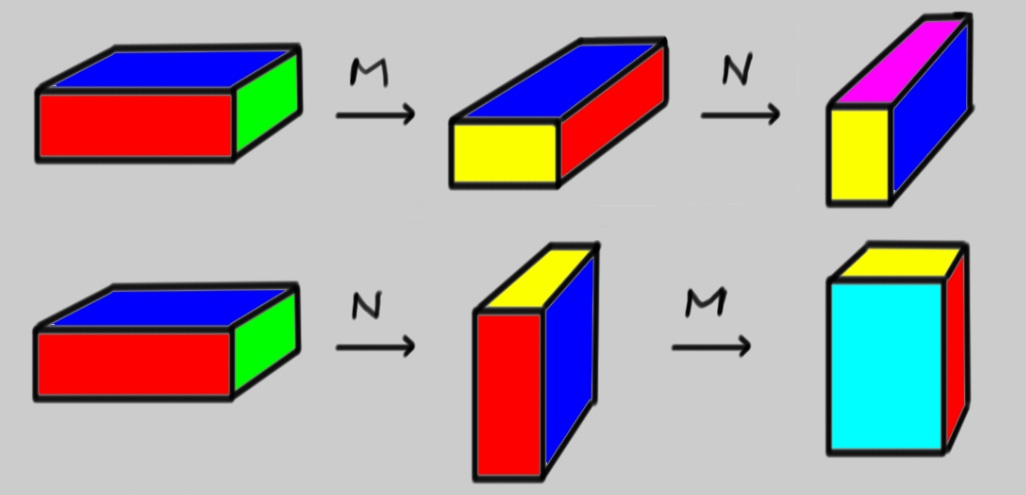
\includegraphics[scale=.3]{MNNM.jpg}
\end{center}
Notice how the end product of $MN$ and $NM$ are different, so $MN\neq NM$ here.
\end{example}

\section*{Trace}\index{Trace}

Matrices contain a great deal of information, so finding ways to extract essential information is useful. Here we need to assume that $n < \infty$ otherwise there are subtleties with convergence that we'd have to address.

\begin{definition}
The \emph{trace} of a square matrix $M=(m_j^i)$ is the sum of its diagonal entries.
\[
\tr M = \sum_{i=1}^{n}m_i^i\, .
\]
\end{definition}

\begin{example}
\[
\tr \begin{pmatrix}
2 & 7 & 6\\
9 & 5 & 1\\
4 & 3 & 8\\
\end{pmatrix} = 2+5+8 = 15
\]
\end{example}
While matrix multiplication does not commute, the trace of a product of matrices does not depend on the order of multiplication:
\begin{align*}
\tr(MN) & = \tr( \sum_l M_l^i N_j^l ) \\
& = \sum_i \sum_l M_l^i N_i^l \\
& = \sum_l \sum_i N_i^l M_l^i \\
& = \tr( \sum_i N_i^l M_l^i ) \\
& = \tr( NM ).
\end{align*}
\videoscriptlink{properties_of_matrices_trace_proof.mp4}{Explanation of this Proof}{scripts_properties_of_matrices_trace_proof}
Thus we have a Theorem:
\begin{theorem} \[\tr(MN)=\tr(NM)\] for any square matrices $M$ and $N$.
\end{theorem}

\begin{example}
Continuing from the previous example, 
\[
M= \begin{pmatrix}
1 & 1 \\
0 & 1 \\
\end{pmatrix}, N=
\begin{pmatrix}
1 & 0 \\
1 & 1 \\
\end{pmatrix}.
\]
so
\[
MN = \begin{pmatrix}
2 & 1 \\
1 & 1 \\
\end{pmatrix} \neq
NM = \begin{pmatrix}
1 & 1 \\
1 & 2 \\
\end{pmatrix}.
\]
However, $\tr(MN) = 2+1 = 3 = 1+2 = \tr(NM)$.
\end{example}

Another useful property of the trace is that:
\[\tr M = \tr M^T\] 
This is true because the trace only uses the diagonal entries, which are fixed by the transpose.  For example:
$\tr \begin{pmatrix}
1 & 1 \\
2 & 3 \\
\end{pmatrix} = 4 = \tr \begin{pmatrix}
1 & 2 \\
1 & 3 \\
\end{pmatrix} = \tr \begin{pmatrix}
1 & 2 \\
1 & 3 \\
\end{pmatrix}^T
$

Finally, trace is a linear transformation from matrices to the real numbers.  This is easy to check.

\videoscriptlink{properties_of_matrices_trace.mp4}{More on the trace function}{scripts_properties_of_matrices_trace}

\begin{remark}[Linear Systems Redux]

Recall that we can view a linear system as a matrix equation
\[MX=V,\] 
with $M$ an $r\times k$ matrix of coefficients, $X$ a $k\times 1$ matrix of unknowns, and $V$ an $r\times 1$ matrix of constants.  If $M$ is a square matrix, then the number of equations~$r$ is the same as the number of unknowns~$k$, so we have hope of finding a single solution.

Above we discussed functions of matrices.  An extremely useful function would be $f(M)=\frac{1}{M}$, where $M\frac{1}{M}=I$.  If we could compute $\frac{1}{M}$, then we would multiply both sides of the equation $MX=V$ by $\frac{1}{M}$ to obtain the solution immediately: $X=\frac{1}{M}V$.

Clearly, if the linear system has no solution, then there can be no hope of finding $\frac{1}{M}$, since if it existed we could find a solution.  On the other hand, if the system has more than one solution, it also seems unlikely that $\frac{1}{M}$ would exist, since $X=\frac{1}{M}V$ yields only a single solution.  

Therefore $\frac{1}{M}$ only sometimes exists.  It is called the \emph{inverse}\index{Inverse matrix!concept of} of $M$, and is usually written $M^{-1}$.
\end{remark}


\section*{References}
Beezer: Part T, Section T
\\
Wikipedia:
\begin{itemize}
\item \href{http://en.wikipedia.org/wiki/Trace_(linear_algebra)}{Trace (Linear Algebra)}
\item \href{http://en.wikipedia.org/wiki/Block_matrix}{Block Matrix}
\end{itemize}

\inputProblems{\propMatricesPath/problems}

